% A simple template for Beamer presentations in LaTeX
% 
% To produce pdf run:
%   $ pdflatex beamer.tex 
%

\documentclass{beamer}
\usetheme{Singapore}

% Bibliography
\usepackage{cite}

\hypersetup{colorlinks=true}

% Show table of contents between sections
\AtBeginSection[]
{
  \begin{frame}
    \frametitle{Table of Contents}
    \tableofcontents[currentsection]
  \end{frame}
}

% Graphics examples
%\centerline{\includegraphics[height=2.5in]{figs/normal.pdf}}
%\includegraphics[width=4in]{figs/makefile.png}

%%%%%%%%%%%%%%%%%%%%%%%%%%%%%%%%%%%%%%%%%%%%%%%%%%%%%%%%%%%%

\begin{document}

\title{Parallel Computing Through Code Analysis}
\date{\today}
\date{10 May 2017}
\author{Clark Fitzgerald}
\institute{UC Davis - Statistics Student Seminar}

\frame{\titlepage}

\begin{frame}
    \frametitle{Outline}
    \tableofcontents
\end{frame}

%%%%%%%%%%%%%%%%%%%%%%%%%%%%%%%%%%%%%%%%%%%%%%%%%%%%%%%%%%%%
\section{Motivation}
%%%%%%%%%%%%%%%%%%%%%%%%%%%%%%%%%%%%%%%%%%%%%%%%%%%%%%%%%%%%
\begin{frame}

    \frametitle{Loop detectors count cars, measuring velocity and
    occupancy}

\centerline{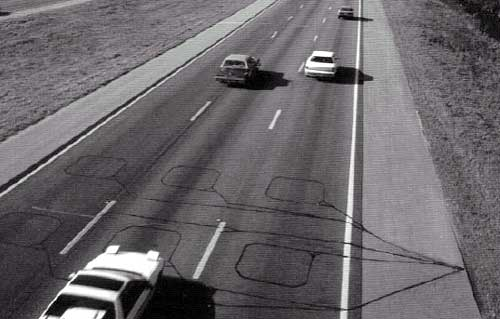
\includegraphics[height=2.5in]{loop_detector.jpg}}

\end{frame}
%%%%%%%%%%%%%%%%%%%%%%%%%%%%%%%%%%%%%%%%%%%%%%%%%%%%%%%%%%%%
\begin{frame}

\frametitle{Caltrans Performance Measurement System (PeMS) records this
data for the whole state}

    \begin{itemize}
        \item Each sensor measures 3 quantities
        \item Every thirty seconds they produce a new data point
        \item $43,680$ sensors in California
    \end{itemize}

    $\implies$  377 million new data points per day

\end{frame}
%%%%%%%%%%%%%%%%%%%%%%%%%%%%%%%%%%%%%%%%%%%%%%%%%%%%%%%%%%%%
\begin{frame}

    \frametitle{Traffic engineers study the relationship between 
    density and flow \cite{li2011fundamental}}

\centerline{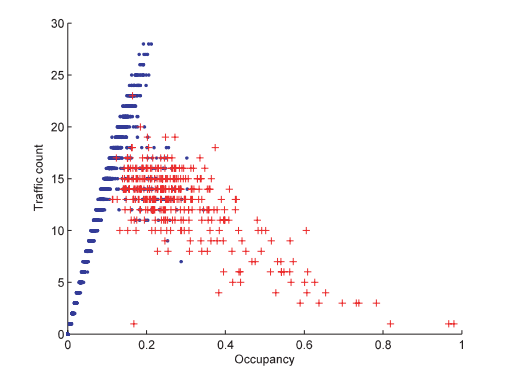
\includegraphics[height=2.5in]{fundamental_diagram.png}}

\end{frame}
%%%%%%%%%%%%%%%%%%%%%%%%%%%%%%%%%%%%%%%%%%%%%%%%%%%%%%%%%%%%
\begin{frame}

    \frametitle{Using more data allows new types of analyses}

    \begin{itemize}
        \item Finding groups of similar detectors
        \item Effect of policy such as speed limits and carpool lanes
        \item Impact of road features such as on/off ramps
        \item Effect of weather
    \end{itemize}

\end{frame}
%%%%%%%%%%%%%%%%%%%%%%%%%%%%%%%%%%%%%%%%%%%%%%%%%%%%%%%%%%%%
\section{Simple example}
%%%%%%%%%%%%%%%%%%%%%%%%%%%%%%%%%%%%%%%%%%%%%%%%%%%%%%%%%%%%
\begin{frame}


\frametitle{Topics}

\begin{itemize}

    \item Why I'm a bad programmer
    \item Introduction to scipy.stats (from Python!)
    \item Live Demo

\end{itemize}

\end{frame}
%%%%%%%%%%%%%%%%%%%%%%%%%%%%%%%%%%%%%%%%%%%%%%%%%%%%%%%%%%%%
\section{Conclusion}
%%%%%%%%%%%%%%%%%%%%%%%%%%%%%%%%%%%%%%%%%%%%%%%%%%%%%%%%%%%%
\begin{frame}


\frametitle{Topics}

\end{frame}
%%%%%%%%%%%%%%%%%%%%%%%%%%%%%%%%%%%%%%%%%%%%%%%%%%%%%%%%%%%%

\begin{frame}
    {\footnotesize
    \bibliographystyle{authortitle1}
    \bibliography{../../citations}
    }
\end{frame}


\end{document}
